% Time form: past tense

\newpage
\section{Variant Decision: AI Integration}\label{sec:variant-decisions-ai-integration}

During the \gls{AI}-research~\ref{sec:ai-research} we identified two interesting ways to allow \gls{NSAK} to interact with \gls{AI} based technologies.
As illustrated in~\ref{fig:ai-integration-variant-1-ai-agent-in-nsak}, the first variant purposes to implement an \gls{AI}-agent directly into the framework and use it in scenarios and drills.
In the second variant shown in~\ref{fig:ai-integration-variant-2-nsak-as-mcp-server}, the capabilities of \gls{NSAK} and other relevant tools on the \gls{NSAK} device would be exposed via \gls{MCP}.

\subsection{Variant 1: AI-agent in NSAK}\label{subsec:variant-decision-ai-integration-variant-1}

\begin{figure}[H]
	\centering
	\includesvg[width=1.0\linewidth]{../assets/diagrams/research/llm_agent_mcp_communications_variant_1.drawio}
	\caption{AI Integration Variant 1: AI-agent in NSAK}
	\label{fig:ai-integration-variant-1-ai-agent-in-nsak}
\end{figure}

\begin{figure}[H]
	\centering
	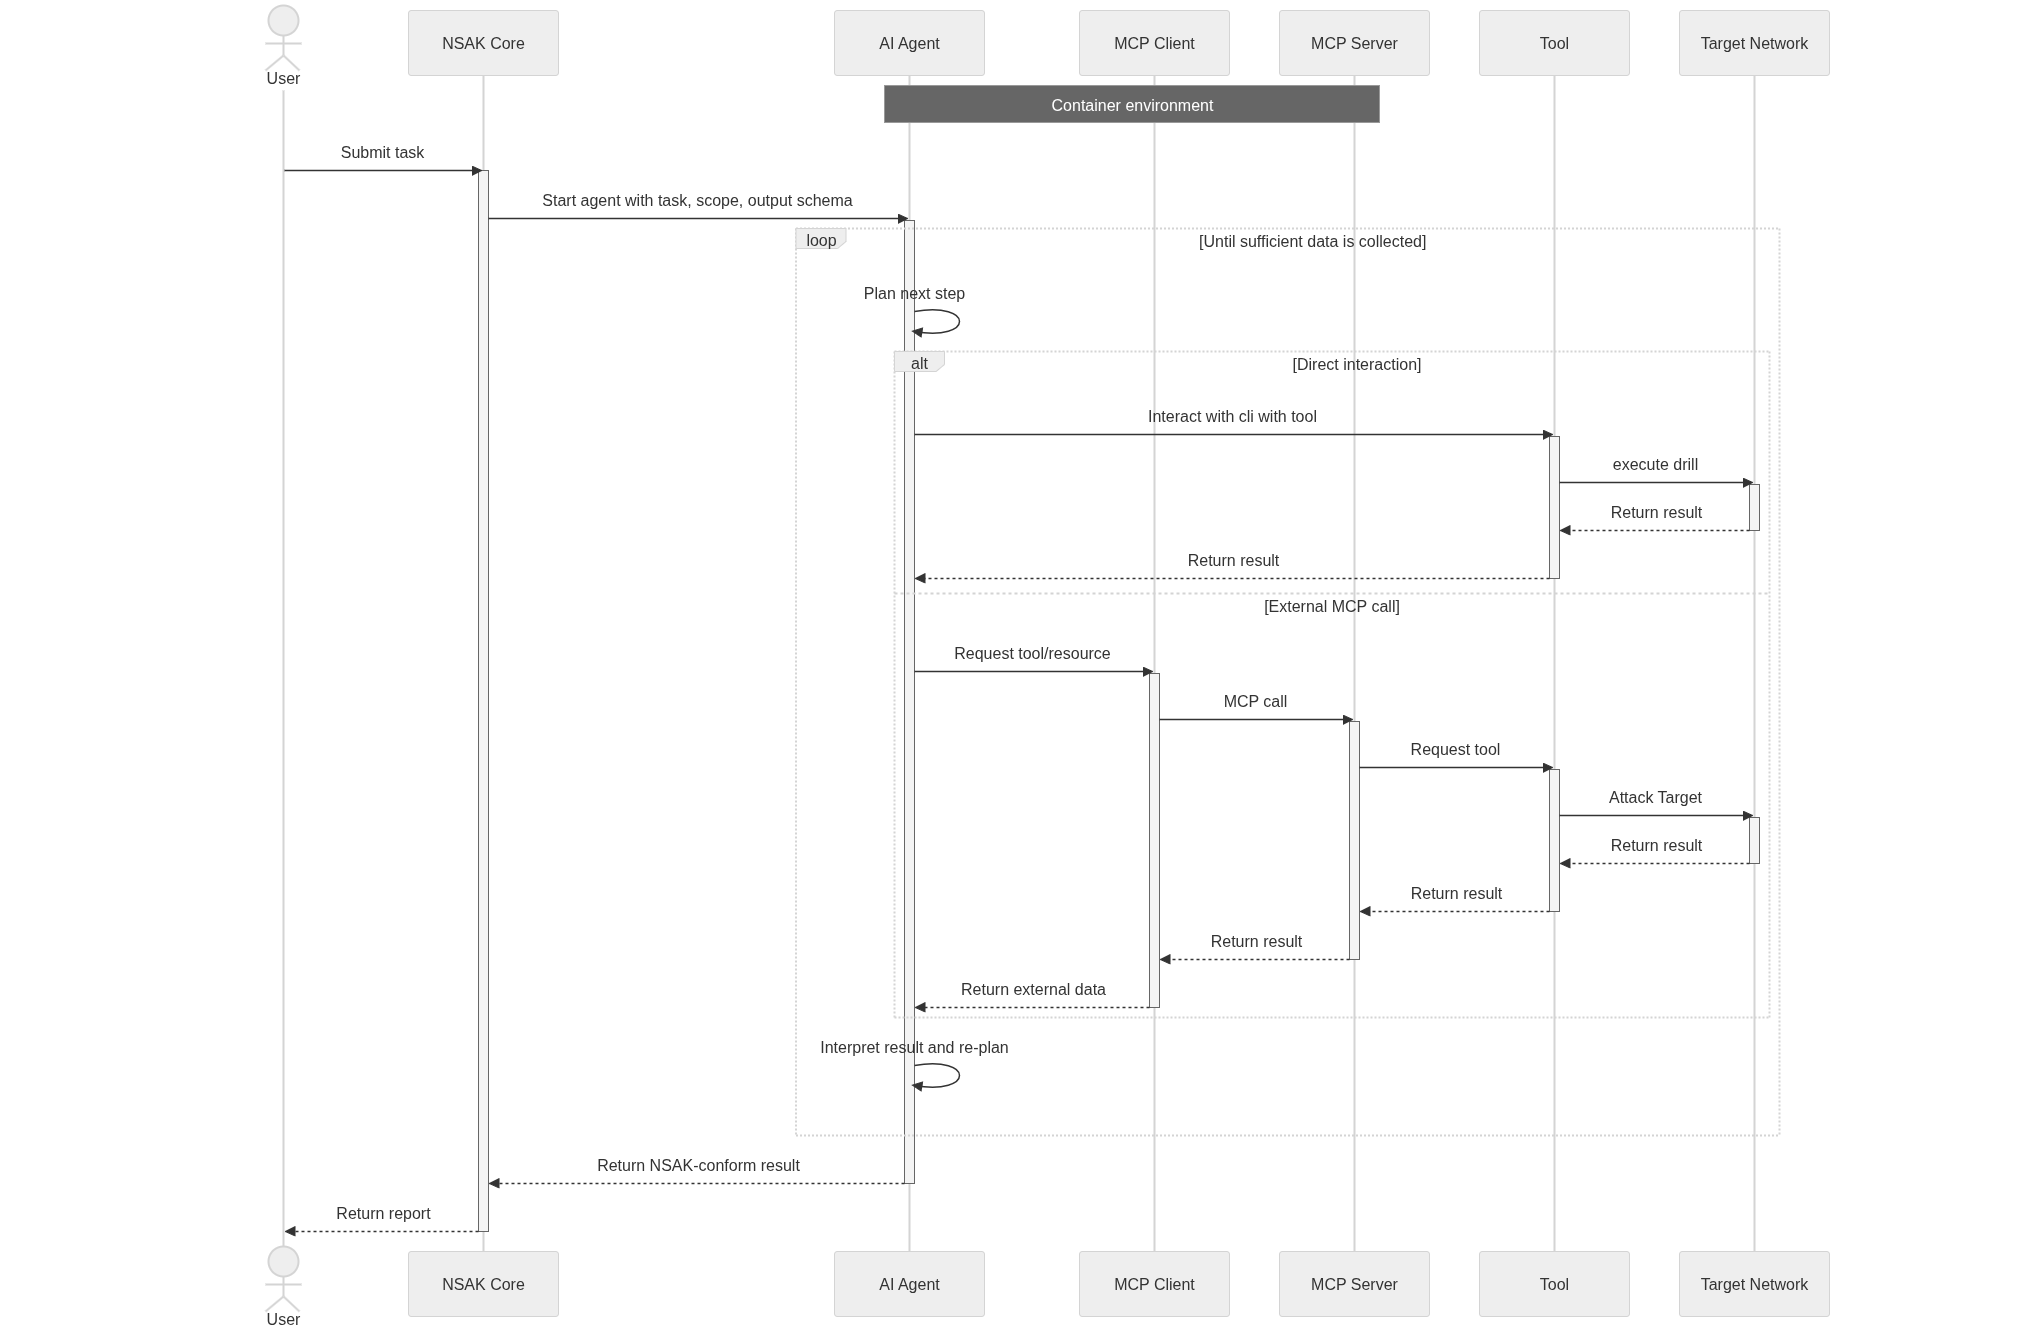
\includegraphics[width=0.7\linewidth]{../assets/diagrams/ai-variants/variant1-internal-agent.drawio}
	\caption{Variant 1, AI Agent in NSAK}
	\label{fig:variant1-internal-agent}
\end{figure}

In this architecture, the \gls{AI} agent is embedded within the \gls{NSAK} device.
The \gls{NSAK} core establishes the operational guardrails and schema, and provides the initial prompt to the \gls{AI AGENT}.
The agent uses a local or remote \gls{LLM}, which is accessible over the management network.
It operates within an iterative loop, in which it may either invoke external tools via a command-line interface (e.g., nmap, Metasploit) or interact with them through an \gls{MCP} server interface.
The results of these operations are subsequently processed and returned to the \gls{NSAK} core in a structured schema-compliant format.

\subsection{Variant 2: NSAK as MCP Server}\label{subsec:variant-decision-ai-integration-variant-2}

\begin{figure}[H]
	\centering
	\includesvg[width=1.0\linewidth]{../assets/diagrams/research/llm_agent_mcp_communications_variant_2.drawio}
	\caption{AI Integration Variant 2: NSAK as MCP server}
	\label{fig:ai-integration-variant-2-nsak-as-mcp-server}
\end{figure}

\begin{figure}[H]
	\centering
	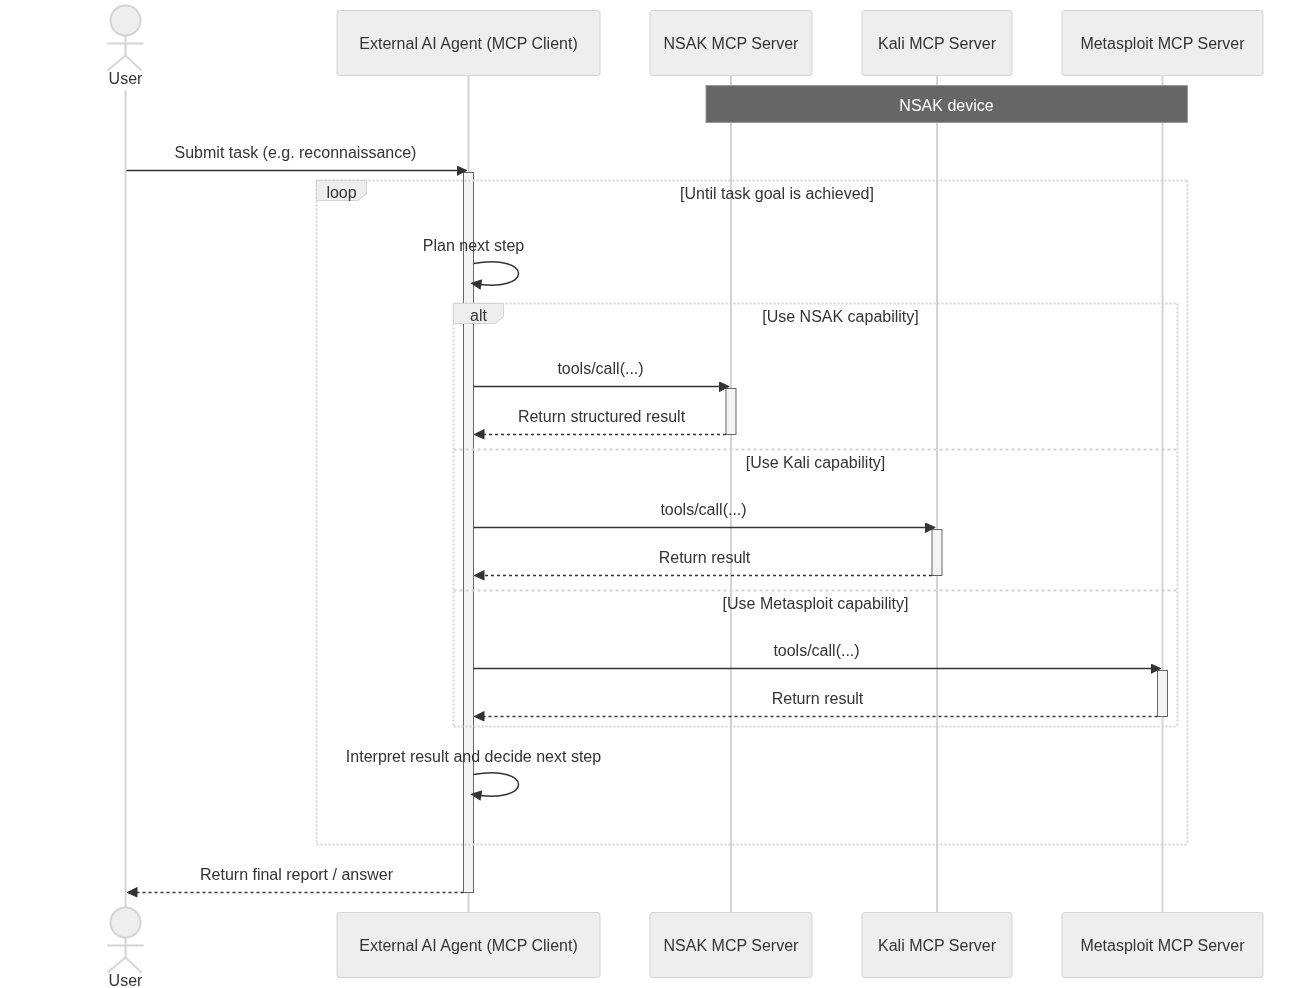
\includegraphics[width=0.7\linewidth]{../assets/diagrams/ai-variants/variant2-external-ai-client.drawio}
	\caption{Variant 2 NSAK MCP Server}
	\label{fig:variant2-external-ai-client}
\end{figure}

Variant 1, in which the \gls{AGENTIC-AI} is embedded within the \gls{NSAK} device, enables the definition and enforcement of schemas and security policies within a controlled environment.
Furthermore, it allows direct interaction with tools via the command-line interface and integration with \gls{MCP} servers.
This results in a tightly coupled architecture with high control and consistency.

In contrast, Variant 2 relies on an external agent that accesses the \gls{NSAK} device through an exposed \gls{MCP} server interface.
While this approach provides increased modularity, it also introduces limitations in flexibility, as the agent is restricted to the set of tools exposed by the \gls{NSAK} device.

From a holistic and multi-layered architectural perspective, Variant 1 is preferred.
It enables deeper system integration, higher security, and a wider range of executable tools.

\subsection{Decision}\label{subsec:variant-decision-ai-integration}

The project team decided in favor of \textbf{Variant 1: AI-agent in NSAK}~\ref{subsec:variant-decision-ai-integration-variant-1}, as it promises to greatly increase the capabilities of \gls{NSAK} regarding autonomy and automation.
